As a prelude, we start with an application of classical Gr\"obner bases that deals with a seemingly infinite problem; here, of course, a recurrence helps to ``control infinity''.  

The Fibonacci sequence $F_n$ ($n= 1, 2, \ldots$) is a \textit{strong divisibility sequence}, in that we have $\gcd(F_n, F_m) = F_{\gcd(n,m)}$; in particular, $F_m$ divides $F_n$ if $m \, | \, n$.  This fact was used by \'Edouard Lucas for Mersenne prime testing.  What can we say, for example, about $F_{3n}/F_n$?  It turns out that there is an identity:
\begin{equation}\label{F3n}
(F_{3n} - 5 F_n^3 - 3 F_n)(F_{3n} - 5 F_n^3 + 3 F_n) = 0,
\end{equation}
which explains explicitly the strong divisibility in this case.   Is it possible to derive this using Gr\"obner bases?  The following Macaulay 2 code does exactly that:
\begin{M2}
\begin{verbatim}
i1: R = QQ[z, x, y, t, MonomialOrder => Eliminate 2]

i2: I = ideal(x + y - z, (x*z - y^2)^2 - 1, t - z^3 - y^3 + x^3)

i3: toString groebnerBasis I

o3 = matrix {{25*y^6-10*y^3*t-9*y^2+t^2, z-x-y, ...
\end{verbatim}
\end{M2}  
The variables $z,x,y,t$ represent $F_{n+1}, F_{n-1}, F_n, F_{3n}$, respectively.  The first polynomial defines the recurrence, the second is Cassini's identity, and the third is Lucas' identity.

One can check that factoring the first polynomial in the list above gives (\ref{F3n}).  Bootstrapping this with extra equations, we can also discover that:
\begin{equation}\label{F5n}
(F_{5n} - 25 F_n^5 - 25 F_n^3 - 5 F_n)(F_{5n} - 25 F_n^5 + 25 F_n^3 - 5 F_n) = 0.
\end{equation}
In turn, these findings incite conjectures and proofs.  
For instance, we leave it to the reader to use modular arithmetic to verify from (\ref{F5n}) that the integer $\frac{F_{5n}}{5F_n}$ always has unit digit $1$ base ten.  
%This is an example of the promise of symbolic computation (with Gr\"obner bases) for the recreational mathematician, but there is more than this possible.

% Anton: I don't know a good graph-coloring problem for infinite graphs.
\iffalse
If you are dealing with an interesting problem, it is likely NP-hard.  Thus, any method that can cut down on the exponential search space and finish in a reasonable amount of time is a success.  

Consider the case of vertex 3-colorings of graphs.  Although exponential in the worst-case \cite[pp. 400]{yap2000fundamental}, Gr\"obner bases methods can be used to check or disprove conjectures in graph theory.  This was outlined theoretically in \cite{bayer1982division}, with success on a moderate-sized example \cite{hillar2008algebraic}, so-called Xu's conjecture \cite{shaoji1990size}, previously proved by other means and in much greater generality \cite{akbari2001kr}.

\begin{figure}
\begin{center}
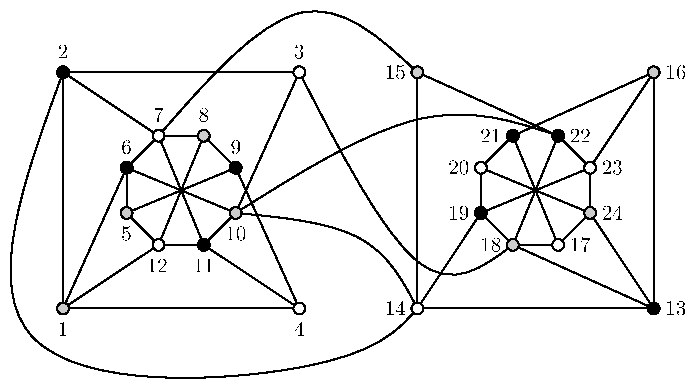
\includegraphics[width=.8 \linewidth]{akbarigraph.pdf}
\caption{Uniquely vertex 3-colorable graph without triangles: a counterexample \cite{akbari2001kr} to Xu's conjecture \cite{shaoji1990size}, which can be proved using Gr\"obner bases \cite{hillar2008algebraic} (see also Problem \ref{graphprob}).}\label{graph}
\end{center}
\end{figure}
\fi

The above is classical.  Here, we are interested  in questions where there are not four or even twenty-four indeterminates, but rather an infinite number of them.  Take for instance the following basic question about ideal membership.  Let $I \subset \mathbb C[x_0,x_1,\ldots]$ be the ideal generated by all permutations acting on the polynomial $f = x_0 x_1 - x_1 x_2^2 +x_1^2$.  Is the following in $I$?
\[ h = x_0 x_4^2 + x_0 x_1^2  +x_1 x_0^2 - 2 x_1 x_0 + x_0 x_3 x_4 - x_0 x_5^2 - x_0 x_3 x_5 - 2 x_1^2.\]

The difference in this question from classical problems of polynomial algebra is that \textit{a priori} there is no guarantee a particular computation, say, with a truncated polynomial ring $\mathbb C[x_0,x_1,\ldots, x_N]$ will do the job.  The following code can give us an answer to our question, however.
\begin{M2}
\begin{verbatim}
i1: needsPackage "EquivariantGB"

i2: R = buildERing({symbol x}, {1}, QQ, 6);

i3: h = x_0*x_4^2+x_0*x_1^2+x_1*x_0^2-2*x_1*x_0+x_0*x_3*x_4- ...

i4: G = egb({x_0*x_1 - x_1*x_2^2 + x_1^2}, Algorithm=>Incremental)

       2       2      2           3      2     2    2         
o4 = {x x  - 2x  + x x  - 2x x , x  - x x , x x  - x  - x x , 
       1 0     1    1 0     1 0   1    1 0   2 0    1    1 0 

                    2           2 
      x x  - x x , x  + x x  - x  - x x }
       2 1    2 0   2    2 0    1    1 0

i5: reduce(h, G)

o5 = 0
\end{verbatim}
\end{M2}  
With the \EGB\ produced above, we can solve ideal membership problems and much more, just as we can use classical Gr\"obner bases in numerous applications.  %Note that arbitrarily large numbers of generators \cite{hillar2008minimal}.  

Developing the machinery to solve such questions is more than an intellectual curiosity.  Basic facts can now be proved by computer such as Theorem~\ref{toric2x2}, but also cutting edge conjectures can be answered using these methods.  For instance, using \cite{EquivariantGB}, it is possible to verify \cite{draisma2013noetherianity, Krone:egb-toric} the first non-trivial case of a basic finiteness conjecture for toric ideals \cite{aschenbrenner2007finite}.  

\begin{theorem}[Proved by computer]\label{monomthm}
For $n > 1$, let $I_n = \ker (y_{ij} \mapsto x_i^2 x_j)$, $1 \leq i \neq j \leq n$.  The invariant chain of toric ideals $I_2 \subset I_3 \subset \cdots$ stabilizes up to the symmetric group.  That is, there is some $N$ such that all elements of $I_m$, $m > N$, are polynomial consequences of relabellings of a finite set of generators of $I_N$.
\end{theorem}

%We note that whether there is always an equivariant Gr\"obner bases is still an open question.

We next list applications of \EGBs\ in rings with infinite numbers of indeterminates.  

\subsubsection{Group theory and Chemistry}

The first use of the concept ``finite up to symmetry" for polynomial rings that we are aware of is in the group theory work of Cohen in \cite{cohen1967laws}.  
Independently, it was problems in algebraic chemistry \cite{ruch1967vandermondesche}, brought to the attention of the authors of \cite{aschenbrenner2007finite} by Andreas Dress, that inspired further applications of asymptotic polynomial algebra in chemistry \cite{Draisma08b}.

\subsubsection{Toric Algebra and Algebraic Statistics}

A big inspiration for asymptotic polynomial algebra comes from the study of certain chains of toric ideals, many of which arise naturally in algebraic statistics.  The series of works \cite{Hillar13, hillar2016corrigendum, draisma2013noetherianity, KKL:equivariant-markov, Krone:egb-toric} have developed fundamental finiteness properties of these structures.  Basic questions remain open, however, as we outline in Section \ref{sec:challenges}.  

In this regard, one of the major motivations for \EGBs\ and infinite symbolic algebra is its application to the problem of sampling from conditional distributions by algebraic methods \cite{diaconis1998algebraic}.  At its essence, the strategy is to find a set of moves through model space that preserves the sufficient statistics of the data.   The idea then is to consider growing families of model classes and show that up to obvious symmetries only a finite set of moves suffices for all infinite numbers of models (e.g., \cite{aoki2003minimal, santos2003higher, hocsten2007finiteness, drton2007algebraic, Draisma08b, Brouwer09e, draisma2009ideals, hillar2012finite, draisma2015finiteness}).  Typically, these moves correspond to elements of a Gr\"obner basis or at least a generating set for some ideal.

\subsubsection{Invariants}
Recently, Nagel and R\"omer~\cite{Nagel} introduced Hilbert series for Noetherian infinite-dimensional rings. Their original theoretical treatment that leads to a proof of rationality of the Hilbert series, in principle, also leads to an effective procedure to compute the series. For an ideal generated up to symmetry by one monomial, such computation was carried out in~\cite{gunturkun2016equivariant}. An alternative approach of~\cite{krone2016hilbert} computes the Hilbert series given an equivariant Gr\"obner basis as the generating function counting words in a regular language.  

\subsection{Finiteness up to symmetry in general}
Although the \EGBs\ described in this article may not directly apply, finiteness up to symmetry plays the central role in the following results (this list is by no means exhaustive).  

It appears in homological stability~\cite{randal2013homological, church2012homological},  the moduli space of $n$ points in a line~\cite{howard2009equations}, geometry as the positivity of the the embedding line bundle grows \cite{ein2012asymptotic}, syzygies of Segre embeddings~\cite{snowden2013syzygies}, Betti tables as their length goes to infinity~\cite{ein2015asymptotics}, tensor geometry~\cite{draisma2014bounded, draisma2015finiteness}, and limiting Grassmannians~\cite{draisma2015plucker}.
Gr\"obner methods have also been used to understand representations of combinatorial categories \cite{sam2016grobner}.


%Anton: This is generally related. Grobner categories -- yes, EGBs in our sense -- no.
% i still like all these -cjh
%\subsubsection{Representation and category theory}
%The theory of FI-algebras \cite{church2014fi, church2015fi} has been developed recently with the symmetric group a central object.  In the direction of different groups other than the symmetric group, there has been work on the general linear group  cite{putman2014representation, sam2016gl}.  
